\section{Motivation} \label{sec:motivation}

%/* Write about the battery drain experiment and how a longer battery life can be achieved by having a longer sleep resp. poll time.*/

\begin{figure}[t]
\centering
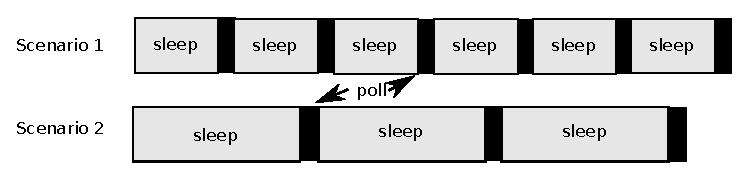
\includegraphics[scale=0.65]{figures/drawing.eps}
\caption{A motivating scenario on the effect of sleep cycle time on energy consumption}
\label{fig:motivating}
\end{figure}

\begin{figure}[t]
\centering
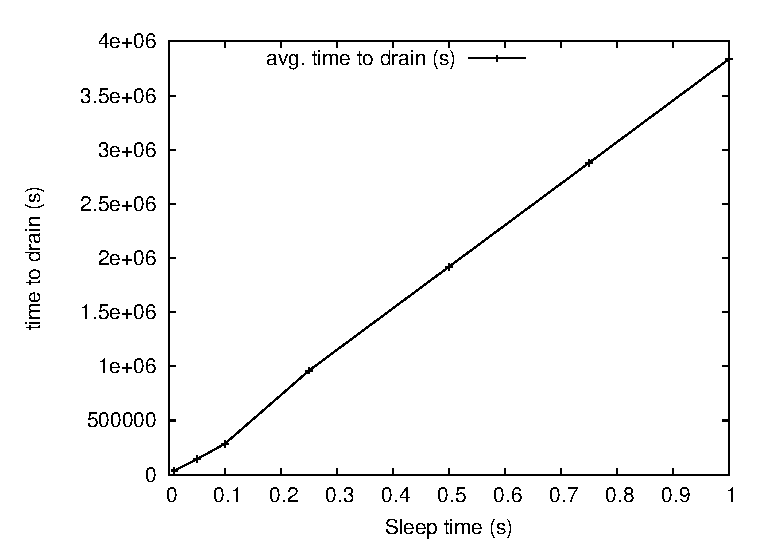
\includegraphics[scale=0.65]{figures/longevity.eps}
\caption{Amount of time required to drain batteries for different sleep cycle times with no workload}
\label{fig:longevity}
\end{figure}

In our project we tackle one of the main challenges in WSNs, namely energy inefficiency. Sensors have a limited amount of power. In the absence of any tasks, a node wastes its energy waiting for transmissions. Making a node sleep (i.e., consume less power) in inactive periods is a well-studied way to mitigates energy waste \cite{1}. However, we consider the effect of the sleep cycle duration on energy consumption. We show a motivating example in Figure~\ref{fig:motivating}. In it we consider two scenarios where no data exist to be received. The first scenario has a sleep cycle duration equal to half of that of the second scenario. The black rectangles denote the period of polling for buffered packets. It is apparent that scenario one consumes more energy since it is switching to poll for received packets more often. The effect of sleep cycle duration extends to scenarios with active receptions and can be intuitively derived. Figure~\ref{fig:longevity} shows the effect of sleep cycle times on the longevity of nodes. It is shown that a sleep time of 1.0 seconds increase longevity by a factor of 10000\% compared to 0.01 seconds.

Given our motivation, the main objective of our work is to maximize sleeping times. However, there is a tradeoff between sleep times and QoS requirements (we consider delay); longer sleep cycle duration translate to larger delay times. A query-based framework is considered for our implementation \cite{2}. We will use ZigBee and IEEE 802.15.4 \cite{3} as our system's infrastructure. The objective of our work is three-fold: First, we will deploy a query-based WSN using Arduino microcontrollers \cite{17} and XBEE modules \cite{18}. Second, we will implement the query-based scheme over QualNet simulator~\cite{16}. Using the deployment and simulation framework we can study the system for the effects of sleep cycle duration on QoS and energy consumption. Third, a mathematical model will be constructed to capture QoS and energy characteristics. From the model, a formula for determining maximum sleeping times is derived. The resulted formula will be tested in the deployment (as a proof-of-concept prototype) and in simulation (to investigate scalability).

The main contribution of our work is to produce a mathematical model that can be used to capture QoS with respect to sleep behavior in WSNs. This model can then be used to derive suitable sleeping times when given certain QoS characteristics and network load. A queueing system \cite{21} can be used to model this problem. An M/G/1 queueing model with vacations \cite{20} is, we claim, suitable for such a problem.

Another challenge is to deploy and simulate a query-based WSN. A full deployment of transaction handling distributively in WSNs would include transaction processing and optimization, routing, aggregation, etc. \cite{2}. We will start with a simple query-based scheme in our deployments. However, we will design it so it would be possible to incrementally develop it to include more transactional features. 
